\documentclass[11pt,a4paper,twoside,openright]{book}

%!TEX root=thesis.tex
\usepackage[
  pdftex,
  plainpages=false,
  colorlinks,
  hyperindex,
  pdfpagemode=UseNone,
  bookmarksopen,
  linkcolor=black,
  citecolor=black,
  urlcolor=black]{hyperref}
\usepackage{graphicx}
\usepackage[boxed]{algorithm}
\usepackage{setspace}
\usepackage{algorithm}
\usepackage{algorithmic}
\usepackage{subfigure}
\usepackage[utf8]{inputenc}
\usepackage[nocompress]{cite}
\usepackage[show]{chato-notes}
\usepackage{booktabs}
\usepackage{enumitem}
\usepackage{amsmath}
\usepackage{mathtools}
\usepackage{url}
\usepackage{listings}
\usepackage{xcolor}

%syntax highlighting for code
\lstset{%
  language=C++,
  basicstyle=\ttfamily,
  keywordstyle=\color{blue}\ttfamily,
  stringstyle=\color{red}\ttfamily,
  commentstyle=\color{green}\ttfamily,
  morecomment=[l][\color{magenta}]{\#}
}

\lstdefinelanguage{XML}{%
  morestring=[b]",
  morestring=[s]{>}{<},
  morecomment=[s]{<?}{?>},
  stringstyle=\color{black},
  identifierstyle=\color{blue},
  keywordstyle=\color{cyan},
  morekeywords={xmlns,version,type}% list your attributes here
}
%end syntax highlighting

\DeclarePairedDelimiter{\ceil}{\lceil}{\rceil}
\graphicspath{{img/}} % Specifies the directory where pictures are stored

\hypersetup{
    unicode=true,          % non-Latin characters in Acrobats bookmarks
    pdftoolbar=true,        % show Acrobats toolbar?
    pdfmenubar=true,        % show Acrobats menu?
    pdffitwindow=false,     % window fit to page when opened
    pdfstartview={FitH},    % fits the width of the page to the window
    pdftitle={My title},    % title
    pdfauthor={Author},     % author
    pdfsubject={Subject},   % subject of the document
    pdfcreator={Creator},   % creator of the document
    pdfproducer={Producer}, % producer of the document
    pdfnewwindow=true,      % links in new window
    colorlinks=true,       % false: boxed links; true: colored links
    linkcolor=black,          % color of internal links
    citecolor=black,        % color of links to bibliography
    filecolor=black,      % color of file links
    urlcolor=black           % color of external links
}
\newcommand{\spara}[1]{\smallskip\noindent{\bf #1}}
\newcommand{\mpara}[1]{\medskip\noindent{\bf #1}}
\newcommand{\para}[1]{\noindent{\bf #1}}

\newtheorem{definition}{Definition}
\newtheorem{proposition}{Proposition}
\newtheorem{property}{Property}
\newtheorem{theorem}{Theorem}
\newtheorem{corollary}{Corollary}
\newtheorem{claim}{Claim}
\newtheorem{example}{Example}
\newtheorem{lemma}{Lemma}
\newtheorem{problem}{Problem}
\newtheorem{assumption}{Assumption}
\newtheorem{observation}{Observation}



\newcommand{\Abs}[1]{\left|#1\right|}
\newcommand{\Tuple}[1]{\left<#1\right>}
\newcommand{\Set}[1]{\left\{#1\right\}}
\newcommand{\List}[1]{\left[#1\right]}
\newcommand{\Paren}[1]{\left(#1\right)}
\newcommand{\Binom}[2]{\left(#1 \atop #2\right)}
\newcommand{\Floor}[1]{\left\lfloor #1 \right\rfloor}
\newcommand{\Ceil}[1]{\left\lceil #1 \right\rceil}
\newcommand{\IntO}[1]{\left(#1\right)}
\newcommand{\IntC}[1]{\left[#1\right]}
\newcommand{\IntLO}[1]{\left(#1\right]}
\newcommand{\IntRO}[1]{\left[#1\right)}
\newcommand{\Choose}[2]{\left( #1 \atop #2\right)}

\newcommand{\sharpP}{{\bf \#P}}
\newcommand{\NP}{$\mathbf{NP}$}
\newcommand{\NPhard}{$\mathbf{NP}$-hard}
\newcommand{\NPcomplete}{$\mathbf{NP}$-complete}
\newcommand{\SPcomplete}{$\mathbf{\#P}$-complete}
\newcommand{\SPhard}{$\mathbf{\#P}$-hard}

\renewcommand{\algorithmicrequire}{\textbf{Input:}}
\renewcommand{\algorithmicensure}{\textbf{Output:}}
\renewcommand{\vec}[1]{\mathbf{#1}}

\usepackage{amssymb}% http://ctan.org/pkg/amssymb
\usepackage{pifont}% http://ctan.org/pkg/pifont
\newcommand{\cmark}{\ding{51}}%
\newcommand{\xmark}{\ding{55}}%

\usepackage{listings} % Source code support
\usepackage{etoolbox}

\lstset{ %
%  backgroundcolor=\color{myBlack},   % choose the background color; you must
  % add \usepackage{color} or \usepackage{xcolor}
  basicstyle=\ttfamily\footnotesize\color{black},        % the size of the fonts
  % that are used for the code
  breakatwhitespace=false,         % sets if automatic breaks should only happen at whitespace
  breaklines=true,                 % sets automatic line breaking
  captionpos=b,                    % sets the caption-position to bottom
%  commentstyle=\color{grey},       % comment style
  deletekeywords={...},            % if you want to delete keywords from the given language
  escapeinside={\%*}{*)},          % if you want to add LaTeX within your code
  extendedchars=true,              % lets you use non-ASCII characters; for 8-bits encodings only, does not work with UTF-8
  frame=single,                    % adds a frame around the code
  keepspaces=true,                 % keeps spaces in text, useful for keeping indentation of code (possibly needs columns=flexible)
  keywordstyle=\color{red},       % keyword style
 % language=go,                 % the language of the code
  morekeywords={*,...},            % if you want to add more keywords to the set
  numbers=left,                    % where to put the line-numbers; possible values are (none, left, right)
  numbersep=5pt,                   % how far the line-numbers are from the code
 % numberstyle=\tiny\color{myGray}, % the style that is used for the
  % line-numbers
%  rulecolor=\color{white},         % if not set, the frame-color may be changed on line-breaks within not-black text (e.g. comments (green here))
  showspaces=false,                % show spaces everywhere adding particular underscores; it overrides 'showstringspaces'
  showstringspaces=false,          % underline spaces within strings only
  showtabs=false,                  % show tabs within strings adding particular underscores
  stepnumber=1,                    % the step between two line-numbers. If it's 1, each line will be numbered
  stringstyle=\color{green},     % string literal style
  tabsize=2,                       % sets default tabsize to 2 spaces
  title=\lstname                   % show the filename of files included with \lstinputlisting; also try caption instead of title
}

\usepackage[toc,page]{appendix}		% appendice
\usepackage{lscape}
 % load packages config
\usepackage{frontmatter} % first page layout and meta

%\linespread{1.2}  % max 1.3
\setstretch{1.3}  % interline spacing. Please set as 1 for drafts.

\begin{document}

% Template settings
\title{PROSIT \\A tool for optimal design of soft-real time systems}
\providecommand{\autore}{Gianluca Bortoli}
\providecommand{\principaladviser}{Prof. Luigi Palopoli}
\providecommand{\annoacc}{2014-2015}

% generate first page
\titlep

% indexes
\frontmatter
\pagenumbering{Roman}
\tableofcontents
%\listoffigures
%\listoftables
%\listofalgorithms

\clearpage
\pagestyle{headings}
\renewcommand{\chaptermark}[1]{\markboth{{\chaptername}\ \thechapter.\hspace{1em}#1}{}}

% ------------------
% TEXT STARTS HERE
% ------------------
\mainmatter

%!TEX root=../thesis.tex
\chapter{Introduction}\label{chp:introduction}

% + what is real-time
% + difference between soft, hard & firm
% + where we can fint them in everyday life

Real-time systems \cite{hardrealtime} is used to describe any information processing system that has to respond to externally generated input stimuli within a finite amount of time. This constraint is called \emph{deadline} and it can be either hard, soft or firm.\\
A deadline is said to be \emph{hard} if a deadline miss causes a critical failure in the system. This is the case of safety-critical applications and other systems in which the result of an operation must be given within the deadline. For example, if the microprocessor, that is the core part of the control unit of our cars, takes too much time to evaluate the distance measured by the parking sensors it will lead to a crash. This event is not admissible since it jeopardizes the driver's safety.\\
On the other hand, \emph{soft} deadlines describe situations in which deadlines are not such strict. The usefulness of the result degrades as time passes after the deadline. The same is valid for the Quality of Service (QoS), but it does not lead to any type of failure or damage. For example, most of the multimedia streaming services are based on this type of deadline, given that the tasks taken into consideration do not put any life at risk.\\
Finally, a deadline is said to be \emph{firm} if a result computed late is completely useless (like hard real-time), leading to a reduction of the QoS (as it happens with soft real-time) but not to a crash. This types of systems can be seen as a sort of mix between the two previous ones.\\
Moreover, it is possible to talk of \textbf{probabilistic deadlines} \cite{abeni} for what concerns \emph{soft} real-time systems. This term is highly related to the QoS and it indicates that the deadline would be met with a given probability. In this sense, deterministic deadlines are considered as a particular case of the probabilistic ones in which the deadline miss probability is zero.\\ 
In this thesis the focus lays on \textbf{soft real-time} tasks. This branch of computer science is continuously gaining popularity, because of the number of embedded devices which have a microprocessor and, in many cases, also a network interface is growing exponentially. In addition to the examples mentioned before, all the electrical applicances we have in our houses are becoming way much smarter than their predecessors, building what is called the Internet of Things.\\
This thesis is structured as follows. In Chapter 2 a formal definition of the problem is given. Chapter 3 presents the PROSIT tool. Chapter 4 is devoted to display some experimental results, while Chapter 5 concludes the thesis.      
%!TEX root=../thesis.tex
\chapter{Problem definition}\label{chp:model}

% + formal task definition
% + periodic, aperiodic and sporadic tasks
% + schedulers
% + define RR and its properties
% + the problem we want to resolve
% + the QoS function
% + markov process background
% - quasi birth-deadth process interpretation
% - the benefits of modeling as QBDP

\section{The task model}
We consider a set of real-time tasks \( \{\tau_{i}\} \) which share a processing unit (CPU), where every tast consists of a stream of jobs \( J_{i,\,k} \).\\
Each job \( j_{i,\,k} \) is defined as a touple \( \left(r_{i,\,k}, \;f_{i,\,k}, \;c_{i,\,k}\right) \) in which:
\begin{itemize}
  \item \( r_{i,\,k} \) is the \emph{release} time for the \( k_{th} \) instance of the \( i_{th} \) task. In other words this is the time in which the job arrives and becomes elegible for execution by the scheduler.
  \item \( f_{i,\,k} \) is the \emph{finishing} time, that is the moment in which the computation for the \( j_{i,\,k} \) ends.
  \item \( c_{i,\,k} \) is the \emph{computation} time, that is the amount of time for which the \( j_{i,\,k} \) was running.
\end{itemize} 

The computation time is assumed to be an independent and identically distributed (i.i.d.\footnote{Two random variables X and Y are said to be i.i.d. if the first has the same probability distribution of the second one and both are mutually indipendent, which means that the occurrence of X does not affect Y (and vice versa).}) stochastic process, since the soft real-time model we are going to explain and use is based on probabilistic deadlines rather than the classic hard deadline.\\
Hence for each \( k \), \( c_{i,\,k} \) is a random variable described by a certain Probability Mass Function (PMF).\\
Every job \( J_{i,\,k} \) has also a relative deadline \( D_{i} \), which is used to define the absolute deadline \( d_{i,\,k} = r_{i,\,k} + D_{i} \). \\
A deadline is respected if \( f_{i,\,k} \leq d_{i,\,k} \) and it is missed if \( f_{i,\,k} > d_{i,\,k} \). In order to be more precise, a probabilistic deadline is respected if \( \Pr\{f_{i,\,k} > r_{i,\,k} + D_{i} \} \leq p_{i} \).

\section{Different type of tasks}
There are three types of tasks: \emph{periodic}, \emph{aperiodic} and \emph{sporadic}.\\
A periodic task has a regular structure and is triggered every period \( T_{i} \). Its lifetime is similar to a cycle in which it activates at time \( r_{i,\,k} \), executes its computation for a period \( c_{i,\,k} \) and then waits the next period to start running again.\\
The second class is composed of these tasks which are not characterize by periodic arrivals. Moreover a minimim interarrival time between different tasks does not exists and, generally speaking, they have not any recurrent structure. They are used to model tasks which occur rarely and have an irregular inner structure.\\
The last type of tasks are very similar to the periodic ones, because both have a minimin interarrival time between each activation, even though it is not always the same. A sporadic task is triggered by an external event which needs the task to be activated, not a timer as happens in for a periodic one.\\
The work which will be described in following chapters takes into consideration only the first two types of tasks.

\section{The scheduler}
The tasks do not run on the bare computer hardware: the Operating System (OS) creates the illusion for each task to have a virtual CPU where they can execute on their own, without the need to share it with anyone else. This gives them the illusion that they are running concurrently and in parallel on the same machine \footnote{This is true if we think of a CPU with one single core. Modern CPUs are multicore, which gives the possibility to actually run multiple tasks at the same time, with an upper bound for the number of process to be executed in parallel given by the number of cores}.\\
Since it is possible to run only one task at a time they need to alternate each other, in order to give everyone the possibility to get their work done. Here is when the \emph{task scheduler} starts its job. The scheduler is responsible for generating a \emph{schedule}, starting from a set of tasks \( \{\tau_{i}\} \).\\
There are several scheduling algorithm which are used to select at every instant \emph{t} which is the task to be executed. More in general a scheduling algorithm \emph{A} generates a schedule \( \sigma_{A}\left(t\right) \) starting from a set of tasks \( \{\tau_{i}\} \).\\
At the end a schedulability test is performed, in which it is checked if the schedule generated by the algorithm \emph{A} guarantees that every deadline (probabilistic or not) is met.\\
There are lots of scheduling algorithm which can be used, such as rate monotonic (RM), earliest deadline first (EDF) and many others, but we concentrated on the \emph{sched\_deadline} algorithm, which is the scheduler currently used in the Linux kernel \footnote{\emph{Sched\_deadline} became the default scheduler from the 3.14 version of the kernel; it is also known as Complete Fair Queuing (CFQ) and it is still the one used in the latest kernel available on \url{www.kernel.org}. The old one was a modified version of the EDF algorithm}.

\section{The Resource Reservation scheduling}
As multiple real-time tasks can run concurrently, this scheduling algorithm allows to associate to a single task \( \tau_{i} \) a \emph{reservation} \( \left(Q_{i}^s,\,Q_{i}^s\right) \).\\ 
This means that the \( i_{th} \) task can execute for \( Q_{i}^s \) time units in every interval of length \( T_{i}^s \). The first value is called \emph{budget} and the second is the \emph{period} of the task.\\
In this way we allocate a fraction of CPU to the task \( \tau_{i} \), which is called \emph{bandwidth}; its is calculated as follows \( B_{i} = \frac{Q_{i}^s}{Q_{i}^s}\).\\
As a consequence, the scheduler reserves for each task its amount of computation time \( Q_{i}^s \) in each period \( T_{i}^s \). It prevents the tasks to run for more time than their budget and therefore each task does not need to take care of what other tasks do while they are executing in parallel.\\
This important propriety for resource reservation (RR) is called \emph{temporal isolation} and it is valid as long as the following scheduling condition holds:
\begin{equation} \tag{1} \label{schedCond}
  \displaystyle\sum_{i} B_{i} =  \displaystyle\sum_{i} \frac{Q_{i}^s}{Q_{i}^s} \leq 1
\end{equation}

This gives us a huge advantage, since we can analyze each task on its own, without careing about what other tasks do at the same time \cite{probGuarantees}.

\section{The quality function}
It is necessary to define also a function which is used to compute the resulting quality of the service, given the scheduling parameters.\\
This function assumes that there exists a dependency between the scheduling parameters and the actual quality. This does not always exists or it can be very difficult to find \cite{prosit}.\\
A possibility is to compute it as a function of the distribution of the delayed tasks. For example, talking about a video streaming sofware, if decoding a frame takes too much time and it leads to miss the deadline, that frame is not displayed and the following job decodes the next frame. Every frame not decoded within the deadline entail a frame not shown on the screen and, consequently, a decrease on the frame rate and on the QoS. 

\section{The problem}
In view of the last considerations, the \emph{analysis} problem we address can be stated as follows: given a series of real-time tasks with a PMF \( U(c) = \Pr\{c_{i,\,j} = c\} \) which describes the stochastic computation time, a PMF \( U(i) = \Pr\{i_{i,\,j} = i\} \) for the interarrival time, a QoS function and the scheduling parameters mentioned so far, say if the set of tasks is schedulable. If it is so, the resulting QoS is computed.\\
For the analysis problem, the scheduling parameters are assumed to be selecred by the designer.

\section{RR modeled as a Markov Chain}
Let me introduce some notations:
\begin{itemize}
  \item \( F_{U}(c) = \displaystyle\sum_{h\,=\,c_{\,min}}^{c} U(c) \) denotes the Cumulative Distribution Function (CDF) for the computation time. For the seek of simplicity, it is assumed that the server period is an integer submultiple of the task period (\( T = NT^{s} \)).
  \item \( d_{k}^{s} \) denotes the latest scheduling deadline used for the job \( J_{k} \). This is an upper bound for \( f_{i,\,k} \): if Equation (\ref{schedCond}) is respected, therefore \( f_{i,\,k} \leq d_{k}^{s} \).
  \item \( \delta_{k} = d_{k}^{s} - r_{k} \) represents an upper bound for the respoinse time of the job.
\end{itemize}

The values \( \delta_{k} \) can take are only in the discrete set of the multiples of the task period and \( \Pr\{\delta_{k} < D\} \) is a lower bound for the prpbability to meet the deadline.\\
The rule \( \delta_{k} \) follows is described in this way \cite{probGuarantees}:
\begin{equation} \tag{2} \label{markovProcess}
\begin{split}
  v_{0} &= c_{0}\\
  v_{k+1} &= max\{0,\,NQ^{s} + c_{k+1}\}\\
  \delta_{k} &= \ceil[\bigg]{\frac{v_{k}}{Q^{s}}}
\end{split}
\end{equation}

The variable \( v_{k} \) cannot be measured empirically, but it is the amount of backlogged computation time that has not be served yet by the scheduler, but it must be taken into account when a new job arrives.\\
Since the computation time for each job is assumed to be an i.i.d. stochastic variable, the the moded shown by Equation \ref{markovProcess} represents a \emph{Discrete-Time Markov Chain} (DTMC).\\
The states of the DTMC are determined by the values \( v_{k} \) can take, while the transitions are the values of the PMF for the computation time \( U(c) \).

\section{The benefits of QBDP}
%!TEX root=../thesis.tex
\chapter{The PROSIT tool}\label{chp:tool}

% - LA BASE DA CUI PARTIRE E' IL PAPER \ref{prosit}
% + struttura dei moduli principali + linguaggio + librerie utilizzate + OOP patterns 
% + use cases diagram (vedi paper) 
% - focus nella creazione dei task RR (qbd_rr_colver.cpp) e di come abbiamo migliorato
%   la creazione della matrice (costruita in 3 fasi separate) in modo da sfruttare a pieno
%   le regolarità presenti al suo interno --> dati su quanto siano migliorate le performance 
%   dopo le modifiche (vedi mail con Bernardo per i numeri)
% - l'approssimazione conservativa della PMF (sia in alto che in basso)
% - distinzione solver da linea di comando e per xml
%     [*] solver_command_line e descrizione parametri in input
%     [*] xml_solver con esempi di chiamata + spiegazione struttura dell'xml da dare in input
% - descrizione web interface e motivi per cui è stata fatta (facilità d'uso per la creazione
%   dell'xml da zero)

\section{Internal structure}
PROSIT is written in C++ and has a modular structure, as an Object Oriented Programming (OOP) implicitly suggests to use.\\
Some external libraries have been used, in order to increase the performance on the matrix operarions and to simplify some other operations. The most important ones are \emph{Eigen}\footnote{\url{http://eigen.tuxfamily.org}}, \emph{TinyXML-2}\footnote{\url{https://github.com/leethomason/tinyxml2}} and \emph{Doxygen}\footnote{\url{http://www.stack.nl/~dimitri/doxygen/}}.\\   
Eigen is the most important library for the core of the tool: it is versatile, because it supports matrices and vectors of all sizes (bot fixed and dynamic) with a lot of matrix operarions already implemented, reliable and very fast, because performance can become a real problem when the matrices have hundreds and hundreds of rows and columns.\\
The second one is TinyXML-2, which has been used as a core part in the parser for the XML file. It provides APIs to accesso to an XML file (which is treated as a Document Object Model) as a C++ object that can be easily browsed and manipulated.\\
The latted is Doxygen, a documentation generator for multiple programming languages. It is widely used in projects\footnote{A list of some projects which already use this tool to generate their documentation is available at \url{http://www.stack.nl/~dimitri/doxygen/projects.html}} because it is highly configurable, it can extract code structure (like class diagrams and so on) even from undocumented files and especially because it is possible to select the output format for the documentation (such as HTML, {\LaTeX} and Unix man pages).\\
The can be devided into standalone modules:
\begin{itemize}
  \item the distribution handler class, for both PMFs and CDFs.
  \item the task descriptor class, in which it is describet the inner structure of a task
  \item the XML parser and the utilities for the XML manipulation.
  \item the probability solver class, which is essentialy a wrapper object for the solving algorithm and the parameters for the RR task.
  \item the QBDP interpretation for the input task; it is the one that actually implements the functions to build the transition matrix and the solution algorithm for the probability solver class.
  \item the QoS function class, which is used to compute the final value for the quality of service, given the input task parameters.
  \item the command line and the XML solver are those which contains the main function that are compiled in order to obtain the executable files.
\end{itemize}

\begin{figure}[H]
  \center{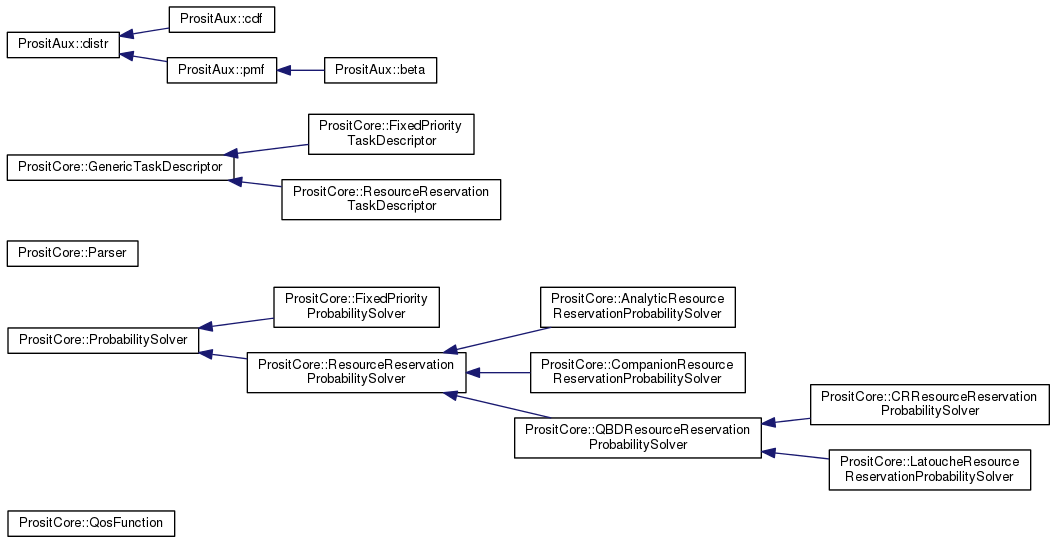
\includegraphics[width=0.9\linewidth]{classdiagram.png}}
  \caption{The PROSIT class diagram generated by Doxygen.}
  \label{automaton}
\end{figure}

\section{Use cases}
The most common use case for the PROSIT tools is the analysis problem: the designer is required to enter the parameters to define the task he/she wishes to analyse.\\
Since a it can only be resource reservation task\footnote{The fixed priority type of task is currently under development and it is not available yet.}, the values for the time requirements (the PMF for the computation time and the one for the interarrival time, if the task is aperiodic) and the scheduling parameters \( Q_{i}^s \) and \( T_{i}^s \) must be provided. Thanks to the temporal isolation property defined in Equation \ref{schedCond}, it allows the tool to treat every task on its own if several tasks are passed as inputs to the tool. The distribution functions can be specified inside the task or taken as input from a file.
\begin{figure}[H]
  \center{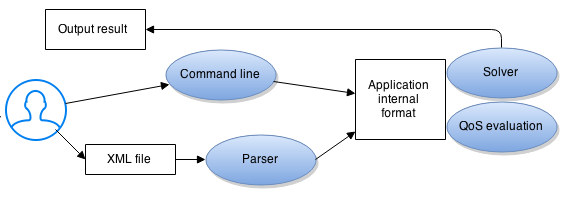
\includegraphics[width=0.7\linewidth]{usecase.png}}
  \caption{The analysis use case for the tool.}
  \label{usecase}
\end{figure}

As a result of a tool invocation, all the provided information are analysed and then the solver for the probabilisti deadlines is called. The \emph{apply\_algorithm()} method called by the probability solver object is a pure virtual function\footnote{Pure virtual functions in C++ are used to take advantage of polymorphism. This is essential for providing a unique interface for multiple objects, which implements different versions of the same method, based on the input selection.}; this allows PROSIT to call the right solution strategy selected by the user.\\
The results and their computation times are printed either on the screen or on a text file.

\section{RR solver}
This solver for resource reservation tasks are based on algorithms for a numerica solution of the relative quasi-birth death process and implements the following methods:
\begin{lstlisting}[frame=bt]
  void pre_process();
  bool compute_pi0();
  void post_process();
  void fill_in_probability_map();
\end{lstlisting}
The \emph{pre\_process()} function creates the matrices used by the QBD algorithms, which are implemented in every sublclass under the name of \emph{apply\_algorithm()}. The second method is responsible of computing the probabilities from the matrix computed earlier. At the end \emph{post\_process()} guarantees that the algorithm gives a reasonable output, while the last method fills the map which is used to display te computation results.\\
The functions described above are called by the solver in the order in which they have been presented.

\subsection{Focus on matrix creation}
The creation of the transition matrix which is later used to apply the algorithms can result in a critical performance bottleneck, since the size can be huge\footnote{Some tests we performed developing the tool calculated the algorithms on a matrix had a size od nearly one thousand.}. Given that the complexity of the algorithms mentioned in Section \ref{benefits} cannot be changed, this will certainly explain the motivation behind the effort to optimize as much as possible the matrix creation phase of the tool.\\
As explained in \ref{transitionmatrix}, the whole transition matrix has a recurrent block structure.\\ 
The first step is to limit the matrix size to the one of \( C \), \( A_{0} \), \( A_{1} \) and \( A_{2} \), since it can be theoretically have an infinite size, which makes it intractable computationally speaking. The values for \( max_{rows} \) and \( max_{cols} \) must be computed first, which are the maximum possible number of rows and columns respectively.\\ 
They can be evaluated as follows: 
\begin{equation*}
\begin{split}
  max_{rows} &= i.get_min() * Q + 1 \\
  max_{cols} &= c.get_max() + 1
\end{split}
\end{equation*}

where \( i.get\_min() \) returns the minimum value for the interarrival time, \( c.get\_max() \) returns the maximum value for the computation time and \( Q \) is the budget associated with the given task.\\
Then, after taking \( max_{v} = max\{max_{rows}\,,\,max_{cols}\} \) as a the size of one of the above mentioned matrices, it is possible to know that the size of the matrix is \( 2 \times max_{v} \).\\
The approach used to calculate the values inside the matrix is based on its internal structure, which is in proven\cite{pipelines} to be like:
\begin{figure}[H]
\begin{equation*} \label{transitionmatrix2}
  P_{i} = 
  \begin{bmatrix}
    a_{i,0} & a_{i,1} & a_{i,H_{i}} & 0 & 0 & 0 & 0 & 0 & 0 & 0 \\
    \vdots & \vdots & \vdots & \vdots & \vdots & \vdots & \vdots & \vdots & \vdots & \vdots\\
    a_{i,0} & a_{i,1} & a_{i,H_{i}} & 0 & \cdots & \cdots & \cdots & \cdots & \cdots & \cdots \\
    b_{i,0,0} & b_{i,0,1} & b_{i,0,H_{i}} & b_{i,0,H_{i}+1} & 0 & \cdots & \cdots & \cdots & \cdots & \cdots \\
    b_{i,0,0} & b_{i,0,1} & b_{i,0,H_{i}} & b_{i,0,H_{i}+1} & b_{i,0,H_{i}+2} & 0 & \cdots & \cdots & \cdots \\
    \vdots & \vdots & \vdots & \vdots & \vdots & \vdots & \ddots & \vdots & \vdots & \vdots \\
    b_{i,G_{i},0} & b_{i,G_{i},1} & \cdots & b_{i,G_{i},H_{i}} & b_{i,G_{i},H_{i}+1} & \cdots & \cdots & b_{i,G_{i},F_{i}} & 0 & \cdots \\
    0 & c_{i,0} & c_{i,1} & \cdots & c_{i,H_{i}} & c_{i,H_{i}+1} & \cdots & c_{i,F_{i}-1} & c_{i,F_{i}} & \ddots \\
    \vdots & \ddots & \ddots & \ddots & \ddots & \ddots & \ddots & \ddots & \ddots & \ddots
  \end{bmatrix}
\end{equation*}
\caption{The transition matrix for the generic \( i^{th} \) stage.}
\end{figure}

In the \( P_{i} \) matrix just described it is possible to spot an internal recurrent configuration, which is highlighted with the different names for the rows \emph{a}, \emph{b} and \emph{c}.\\
To take advantage of this proprerty, the \emph{pre\_process()} method builds the matrix in three steps: the first one is to calculate only the first \emph{a}-row block and then copy its value througout the rest of the first block. Secondly all the \emph{transient}\footnote{This part of the matrix exists only if the task is aperiodic. In the case of a periodic one, this part of the matrix does not exists and the transition matrix is composed only of the \emph{a} and \emph{c} blocks.} rows denoted with the letter \emph{b} are calculated, cell by cell. In the \emph{c} block, as happened for the first one, only the first row is calculated and then it is copied to the following one shifted right by one.
%!TEX root=../thesis.tex
\chapter{Testing and experimental data}\label{chp:experiments}

% + behaviour with changing bandwidth -> analytical vs. CR results (see paper)
% + deep code restructure from original tool to v2.0
% + test to check that the new version of the tool gives correct results
%   comparing them with the ones obtained with the old tool on the same input
% - performance enhencment in matrix creation (see Bernardo's emails) [rememer to put reference
%   in the prosit overview chapter]

Thie version of PROSIT described in this thesis brought a lot of improvements in the project structure, especially in the core classes that holds the inner task structure. Big changes in the code structure imply a complete revision of the results, even though they have been deeply checked in the "old" version of the tool.\\
This decision was not painless at all but is was necessary: PROSIT have been firstly developed and used in some papers\footnote{An example of paper which involved PROSIT to compute the results the authors needed is \cite{probGuarantees}.} and the code structure was not an absolute priority. Then PROSIT gained interest, due to its capability to provide a good abstraction for many of the foundamental concepts in the real-time systems design.\\
The code restructured made it necessary to check that the results provided by the "new" version of the tool does not contain any error. This phase of testing has been done running multiple tasks with different parameters on both versions and then checking the correctness of the results. Comparing the outputs it has not been found any inconsistency.\\
The process of testing and comparison described above was done in an automated way using some bash scripts.

\section{Cyclic Reduction accuracy}
In order to compare the accuracy between the analytical result and the output given by the cyclic reduction (CR) algorithm. This was done considering a task with the same parameters except for the bandwith value. The \( Q_{s} \) value is changed to make the bandwith value in the range [35\% - 60\%]. The results of this comparison is visible in Table .
\begin{table}[H]
\label{comparison}
\begin{center}
\begin{tabular}{| l | l | l | l | l | l |}
  \hline
  Bandwith & 35\% & 40\% & 45\% & 50\% & 60\% \\ \hline
  Analitic bound & 0.602 & 0.809 & 0.906 & 0.956 & 0.991 \\
  CR algorithm & 0.773 & 0.878 & 0.929 & 0.965 & 0.992 \\ \hline
\end{tabular}
\caption{Probabilities for different bandwith and a 50\,\( \mu{s} \) scaling factor.}
\end{center} 
\end{table}

The gap between the results outputted by the two different solving algorithms is significant in the first two columns, but it constantly reduces as the bandwith increases. A bandwith value lower than 40\% gives a probability result smaller than the 80\% that the deadline will be met, which is not sufficient for most of the real-time applications.\\
This means that the CR works preatty well in \emph{heavy-traffic} conditions, namely a situation in which the system is heavily used and it is stressed by many tasks.

\section{Performance enhencment in matrix creation} \label{matrixperformance}
As described in Section \ref{matrixcreation}
%Computing Matrix Size: 442
%elapsed time NEW: 71413 us
%elapsed time OLD: 121238 us
%new method is 49825 us (~40%) faster
%!TEX root=../thesis.tex
\chapter{Conclusion and future work}\label{chp:conclusion}

% + enhencments on web gui: 
%   [+] user authentication so that every user has its own space and computation power on 
%       the server
% + implement solving algorithms described in "Stochastic Analysis of Periodic Real-Time Systems"
% + try to introduce multithreading in some parts, if possible, for performance boost
% + talk about the possible future of this tool (to be published and available to everyone)

The tool presented in this thesis shows how it is possible to improve the design and the analisys phase of soft real-time systems. As a result PROSIT can be employed especially in academic researche, but a use in other fields is not excluded.\\
Possible future enhancements can include some improvements in the web GUI, such as user authentication, and implement some complex but efficient algorithms to solve quasi birth-death processes described in \cite{futurework}. This would make the tool more complete and usable for further research applications.\\
Another possibility is to try introducing multithreading where it is feasible in order to enhence the overall performance of the tool.\\
It is possible to affirm that this is certainly a solid starting point for those who will work and contribute to the PROSIT project in the future.      

%\pagestyle{plain}
\renewcommand{\chaptermark}[1]{\markboth{{\appendixname}\ \thechapter.\hspace{1em}#1}{}}

%\appendix
%\input{sections/appendix.tex}

%\clearpage
%\addcontentsline{toc}{chapter}{References}
\bibliographystyle{plain}
\bibliography{bibliography}

\end{document}